\documentclass[11pt, a4paper]{article}

% --- Packages ---
\usepackage[utf8]{inputenc}
\usepackage[T1]{fontenc}
\usepackage{geometry}
\geometry{top=1in, bottom=1in, left=1in, right=1in}
\usepackage{xcolor}
\usepackage{listings}
\usepackage{hyperref}
\usepackage{minted}
\usepackage{mdframed}
\usepackage{graphicx}
\usepackage{tikz}

% --- Code Listing Styling ---
\definecolor{codegreen}{rgb}{0,0.6,0}
\definecolor{codegray}{rgb}{0.5,0.5,0.5}
\definecolor{codepurple}{rgb}{0.58,0,0.82}
\definecolor{backcolour}{rgb}{0.95,0.95,0.96}

\lstdefinestyle{mystyle}{
    backgroundcolor=\color{backcolour},
    commentstyle=\color{codegreen},
    keywordstyle=\color{blue},
    numberstyle=\tiny\color{codegray},
    stringstyle=\color{codepurple},
    basicstyle=\ttfamily\footnotesize,
    breakatwhitespace=false,
    breaklines=true,
    captionpos=b,
    keepspaces=true,
    numbers=none,
    numbersep=5pt,
    showspaces=false,
    showstringspaces=false,
    showtabs=false,
    tabsize=4
}
\lstset{style=mystyle}

\usetikzlibrary{shapes.geometric, arrows, positioning, fit, backgrounds}

% Define styles for the diagram elements
\tikzset{
    box/.style={rectangle, rounded corners, minimum width=3cm, minimum height=1.5cm, align=center, draw=black, fill=gray!10},
    cloud/.style={draw, ellipse, fill=blue!10, minimum height=1em, align=center},
    arrow/.style={thick,->,>=stealth}
}

\title{\textbf{Lab Exercise 2: Network I/O and Zero-Copy}}
\author{Gianmaria Del Monte}
\date{}

\begin{document}

\maketitle

\section*{Background}
In this exercise, we shift our focus from local disk I/O to the network. Moving massive amounts of data from a storage disk to a network socket using traditional POSIX \texttt{read()} and \texttt{write()} calls suffers from the ``Double Copy'' problem and the ``Syscall Tax.'' 

We will simulate a High-Energy Physics storage node serving a 1GB dataset to a remote client. You have been provided with a naive server implementation and a dummy client. Your task is to profile the baseline performance, and then rewrite the server to utilize advanced Linux I/O techniques to eliminate the bottlenecks.

\begin{figure}[h]
    \centering
    % \resizebox dynamically shrinks the diagram so it never spills over the page margins!
    \resizebox{\textwidth}{!}{%
    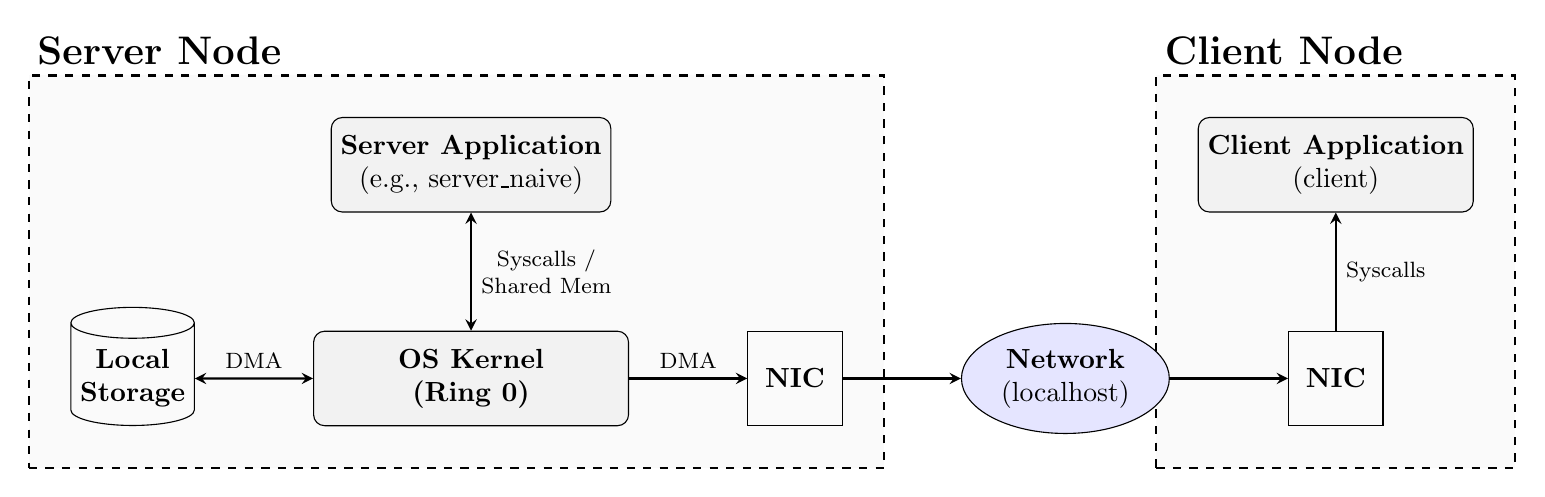
\begin{tikzpicture}[
        % Define standard spacing
        node distance=1.5cm and 1.5cm,
        % Define styles
        box/.style={rectangle, rounded corners, minimum width=2.5cm, minimum height=1.2cm, align=center, draw=black, fill=gray!10},
        cloud/.style={draw, ellipse, fill=blue!10, minimum height=1.2cm, align=center},
        arrow/.style={thick, ->, >=stealth},
        darrow/.style={thick, <->, >=stealth},
        lbl/.style={font=\footnotesize, align=center} % Smaller font for the arrow text
    ]

        % --- Server Node Components ---
        \node (kernel) [box, minimum width=4cm] {\textbf{OS Kernel} \\ \textbf{(Ring 0)}};
        \node (server_app) [box, above=1.5cm of kernel] {\textbf{Server Application} \\ (e.g., server\_naive)};
        \node (disk) [cylinder, draw, shape border rotate=90, aspect=0.25, minimum width=1.5cm, minimum height=1.5cm, align=center, left=1.5cm of kernel] {\textbf{Local} \\ \textbf{Storage}};
        \node (nic) [rectangle, draw, minimum width=1.2cm, minimum height=1.2cm, align=center, right=1.5cm of kernel] {\textbf{NIC}};

        % Server Connections
        \draw [darrow] (server_app) -- node[right, lbl] {Syscalls / \\ Shared Mem} (kernel);
        \draw [darrow] (disk) -- node[above, lbl] {DMA} (kernel);
        \draw [arrow] (kernel) -- node[above, lbl] {DMA} (nic);

        % --- Network ---
        \node (network) [cloud, right=1.5cm of nic] {\textbf{Network} \\ (localhost)};
        \draw [arrow] (nic) -- (network);

        % --- Client Node Components ---
        \node (client_nic) [rectangle, draw, minimum width=1.2cm, minimum height=1.2cm, align=center, right=1.5cm of network] {\textbf{NIC}};
        \node (client_app) [box, above=1.5cm of client_nic] {\textbf{Client Application} \\ (client)};
        
        % Client Connections
        \draw [arrow] (network) -- (client_nic);
        \draw [arrow] (client_nic) -- node[right, lbl] {Syscalls} (client_app);

        % --- Bounding Boxes (using the 'fit' library) ---
        \begin{scope}[on background layer]
            % Server Box: Automatically wraps around the app, kernel, disk, and nic!
            \node (server_box) [draw, dashed, thick, inner sep=15pt, fill=black!2, fit=(server_app) (kernel) (disk) (nic)] {};
            \node [above right, font=\Large\bfseries] at (server_box.north west) {Server Node};
            
            % Client Box: Automatically wraps around the app and nic!
            \node (client_box) [draw, dashed, thick, inner sep=15pt, fill=black!2, fit=(client_app) (client_nic)] {};
            \node [above right, font=\Large\bfseries] at (client_box.north west) {Client Node};
        \end{scope}

    \end{tikzpicture}%
    }
    \caption{Architecture of Lab Exercise 2, illustrating Server and Client Nodes connected via Localhost Network.}
    \label{fig:lab_architecture}
\end{figure}

\section*{Part 1: Environment Setup}
Open your terminal, navigate to the second exercise folder in the course repository, and generate the 1GB dummy dataset:

\begin{minted}{shell}
    cd icscexercises/exercise2
    dd if=/dev/urandom of=1GB_dataset.bin bs=1M count=1024
\end{minted}

Ensure you have the \texttt{liburing} development headers installed on your system (e.g., \texttt{sudo apt install liburing-dev} or \texttt{sudo pacman -S liburing}), as you will need them for Task 3.

\section*{Part 2: The Baseline (Naive I/O)}
Look at the provided \texttt{server\_naive.c} code. It accepts a connection, reads from the disk into a user-space buffer, and writes to the socket.

\begin{enumerate}
\item Compile with \texttt{make}.
\item Start the server wrapped in \texttt{strace} to count the system calls:
\begin{minted}{shell}
    strace -c ./server_naive
\end{minted}
\item Open a second terminal in the folder \texttt{icscexercises/exercise2} and start the client wrapped in the time utility to measure CPU time:
\begin{minted}{shell}
    time ./client
\end{minted}
\end{enumerate}

\textit{Observe the results in Terminal 1 when the transfer finishes. How many thousands of \texttt{read} and \texttt{write} calls were executed?}

\section*{Part 3: Zero-Copy with \texttt{sendfile}}
Create a new file called \texttt{server\_sendfile.c}. Copy the connection logic from the naive server, but replace the \texttt{read/write} loop entirely with the \texttt{sendfile()} system call.

\subsubsection*{Implementation Hints:}
\begin{itemize}
    \item You will need to include \texttt{<sys/sendfile.h>}.
    \item The signature is: \texttt{ssize\_t sendfile(int out\_fd, int in\_fd, off\_t *offset, size\_t count);}
    \item Unlike \texttt{read/write}, you do not need to allocate a \texttt{malloc} buffer! The kernel will route the data directly from the Page Cache to the Network Interface Card (NIC).
    \item Example usage to send 1GB:
\end{itemize}

\begin{minted}{c}
    off_t offset = 0;
    size_t bytes_to_send = 1073741824; // 1 GB
    sendfile(client_socket, file_fd, &offset, bytes_to_send);
\end{minted}

Compile your code. Run your new \texttt{server\_sendfile} through \texttt{strace -c}, triggering the client exactly as you did in Part 2. 

\textit{Observe your new metrics. You should see those thousands of \texttt{read/write} system calls vanish, replaced by just one \texttt{sendfile} call!}

\section*{Part 4: Zero-Copy Pipelines with \texttt{splice}}
While \texttt{sendfile} is fantastic, it was historically limited: the output file descriptor \textit{had} to be a network socket. What if we want to do zero-copy between two regular files, or a file and a hardware device? 

The Linux kernel provides a more flexible zero-copy mechanism called \texttt{splice()}. It allows you to move data between any two file descriptors, as long as one of them is a kernel pipe. By creating a pipe, we can build an in-kernel pipeline: Disk $\rightarrow$ Pipe $\rightarrow$ Socket, completely bypassing user-space memory!

Create a new file called \texttt{server\_splice.c}. Copy the connection logic from the naive server, but replace the \texttt{read/write} loop entirely with a \texttt{splice()} pipeline.

\subsubsection*{Implementation Hints}
\begin{itemize}
    \item You must add \texttt{\#define \_GNU\_SOURCE} at the \textbf{very top} of your C file (before any \texttt{\#include}) to unlock Linux-specific pipe features.
    \item You will need to include \texttt{<fcntl.h>}.
    \item Create a kernel pipe before your loop: \texttt{int pipefds[2]; pipe(pipefds);}
    \item \textbf{The Pipe Bottleneck:} Standard Linux pipes hold exactly 64KB. If you loop this, you will execute over 32,000 \texttt{splice} calls! To fix this, resize your pipe to 1MB before the loop: \\
    \texttt{fcntl(pipefds[0], F\_SETPIPE\_SZ, 1024 * 1024);}
    \item The signature is: \texttt{ssize\_t splice(int fd\_in, off\_t *off\_in, int fd\_out, off\_t *off\_out, size\_t len, unsigned int flags);}
    \item Inside your loop, you will need \textbf{two} \texttt{splice} calls. 
    \begin{enumerate}
        \item Splice data from the \texttt{file\_fd} into the write-end of the pipe (\texttt{pipefds[1]}).
        \item Splice data from the read-end of the pipe (\texttt{pipefds[0]}) directly into the \texttt{client\_fd}.
    \end{enumerate}
    \item You can pass \texttt{NULL} for the offsets to let the kernel update them automatically, and use \texttt{SPLICE\_F\_MORE} for the flags.
\end{itemize}

Compile your code. Run your new \texttt{server\_splice} through \texttt{strace -c}, triggering the client. 

\textit{Observe your metrics. You should see zero \texttt{read} or \texttt{write} calls, replaced entirely by \texttt{splice}. You have successfully built a zero-copy pipeline!}

\section*{Bonus Task 1: The Future with \texttt{io\_uring}}
Create a file called \texttt{server\_uring.c}. In the lecture, we discussed how \texttt{io\_uring} can batch operations and execute them asynchronously. 

We will use a feature called \textbf{I/O Chaining} (\texttt{IOSQE\_IO\_LINK}). We will instruct the kernel to read a large chunk of data, and if successful, immediately write it to the socket, all without waking up the application!

\subsubsection*{Implementation Hints:}
\begin{itemize}
    \item Include \texttt{<liburing.h>}.
    \item Allocate a large buffer (e.g., 256MB) to process the transfer in chunks.
    \item Initialize the ring, queue the requests, and submit them with a \textit{single} system call:
\end{itemize}

\begin{minted}{c}
    struct io_uring ring;
    io_uring_queue_init(8, &ring, 0);

    // 1. Get an SQE and prepare the READ operation
    struct io_uring_sqe *sqe1 = io_uring_get_sqe(&ring);
    io_uring_prep_read(sqe1, file_fd, buffer, chunk_size, offset);

    // Set the LINK flag! This tells the kernel
    // "Do the next SQE immediately after this one"
    io_uring_sqe_set_flags(sqe1, IOSQE_IO_LINK);

    // 2. Get the next SQE and prepare the WRITE operation
    struct io_uring_sqe *sqe2 = io_uring_get_sqe(&ring);
    io_uring_prep_write(sqe2, client_socket, buffer, chunk_size, 0);

    // 3. Submit both operations to the kernel with ONE system call
    io_uring_submit(&ring);

    // 4. Wait for the completion queue entries (CQEs) to verify success...
    struct io_uring_cqe *cqe;
    io_uring_wait_cqe(&ring, &cqe);
    // Mark this CQE as seen so the kernel can recycle the slot
    io_uring_cqe_seen(&ring, cqe);

    // Notice that we expect 2 completions (one for read and one for write)
\end{minted}

\subsection*{Lab Question}

\noindent In Part 2, \texttt{strace} revealed that the naive server executed tens of thousands of system calls to transfer the 1GB file. In Part 3, the \texttt{sendfile} implementation accomplished the same transfer with only a few system calls. Based on the lecture, explain what happened to the user-space buffer, and describe the path the data takes from the disk to the network socket when using \texttt{sendfile}.

\vspace{0.2cm}
\noindent
\fbox{
    \begin{minipage}{0.97\textwidth}
        \vspace{4.0cm} 
        \hfill
    \end{minipage}
}

\section*{Bonus Task 2: The Zero-Copy Pipeline}

In Question 2, you hopefully realized a major flaw in our \texttt{io\_uring} implementation: by routing the data through a \texttt{malloc}'d buffer, we still suffered from the Double Copy problem! We eliminated the system call tax, but forced the CPU to copy 2 Gigabytes of memory (1GB up to user space, 1GB down to the socket).

To achieve Zero-Copy I/O, we must keep the data entirely inside the kernel. Because \texttt{io\_uring} does not currently have a dedicated \texttt{sendfile} opcode, we must construct our own in-kernel pipeline using the \texttt{splice()} operation and a kernel pipe.

\subsubsection*{Implementation Hints:}
\begin{itemize}
    \item You must add \texttt{\#define \_GNU\_SOURCE} at the \textbf{very top} of your file (before any \texttt{\#include}) to unlock Linux-specific pipe features.
    \item Delete the user-space buffer allocation entirely.
    \item Create a kernel pipe before your loop: \texttt{int pipefds[2]; pipe(pipefds);}
    \item \textbf{The Pipe Bottleneck:} Standard Linux pipes hold exactly 64KB. If you loop this, you will have to call \texttt{io\_uring\_submit} over 16,000 times for a 1GB file, bringing back the Syscall Tax! To fix this, resize your pipe to 1MB before the loop: \\
    \texttt{fcntl(pipefds[0], F\_SETPIPE\_SZ, 1024 * 1024);}
    \item Change your \texttt{CHUNK\_SIZE} to \texttt{1024 * 1024} (1MB). 
    \item Replace \texttt{io\_uring\_prep\_read} with \texttt{io\_uring\_prep\_splice}. You will splice data from the \texttt{file\_fd} into the write-end of the pipe (\texttt{pipefds[1]}). The offset for a pipe must be \texttt{-1}. Set the \texttt{IOSQE\_IO\_LINK} flag just like before!
    \item Replace \texttt{io\_uring\_prep\_write} with another \texttt{io\_uring\_prep\_splice}, moving data from the read-end of the pipe (\texttt{pipefds[0]}) directly into the \texttt{client\_fd}.
\end{itemize}

Compile and run your new server with \texttt{strace -c}. You have successfully built a pipeline where the data never leaves Ring 0!

\vspace{0.5cm}
\hrule
\vspace{0.5cm}

\subsection*{Beyond the Exercise: True Zero-Copy and Zero-Syscall}
Even with our 1MB pipe, \texttt{strace} will show about 1,024 calls to \texttt{io\_uring\_enter}. We mitigated the Syscall Tax, but we didn't eliminate it. Furthermore, data is still moving from the Page Cache into a Pipe buffer before hitting the socket. 

To achieve absolute maximum performance in modern Linux, systems engineers use two advanced techniques:

\begin{enumerate}
    \item \textbf{SQPOLL:} \texttt{io\_uring} can be initialized with the \texttt{IORING\_SETUP\_SQPOLL} flag. This tells the kernel to spawn a dedicated background thread that constantly polls your Submission Queue in shared memory. You never have to call \texttt{io\_uring\_submit()} again; you just put the work in memory, and the kernel thread executes it automatically!
    \item \textbf{mmap + send\_zc:} Instead of using pipes, you can \texttt{mmap()} the file into your virtual memory space, and then use \texttt{io\_uring\_prep\_send\_zc} (Zero Copy send). The kernel pins the memory and instructs the Network Interface Card (NIC) to use DMA to pull the data directly from the Page Cache to the network wire. The CPU doesn't copy a single byte.
\end{enumerate}

\end{document}